\documentclass{article}
\usepackage[utf8]{inputenc}
\usepackage[english]{babel}
\usepackage{amsmath}% http://ctan.org/pkg/amsmath
\usepackage{listings}
\usepackage{graphicx}
\usepackage{comment}
\usepackage{float}
\usepackage{biblatex}
\usepackage{lscape}
\usepackage{csquotes}
\usepackage{multirow}
\usepackage{float}
\usepackage{caption}
\usepackage{hyperref}
\usepackage{longtable} 

\addbibresource{bibliography.bib}
\usepackage[a4paper,pdftex,bottom=20mm, width=160mm]{geometry} % A4paper margins
\setlength{\parindent}{0pt} % Tar bort indenteringen på paragrafer 
\setlength{\parskip}{1em}

%tar bort linebreaks "i ord"%
\tolerance=1
\emergencystretch=\maxdimen
\hyphenpenalty=10000
\hbadness=10000
%------%

%Integration of Git for version control%




\title{

\includegraphics[scale=1.5]{liu_logga.png} \\
\vspace{2.0cm} \textbf{Customer Requirements Specification} \\
 \endgraf\rule{\textwidth}{.4pt}
  \large \textbf{TDDC88 - Project}\\
 
   }
   
   
\author{William Eriksson, Alina Wåhlberg, Gustav Gaunitz \& Melker Forsberg}

\date{\today} 

\begin{document}

\maketitle
\newpage
```latex
\section{Document Change History}

\begin{center}
\small\textit{Note: This change history table was generated by Autoleaf AI under the supervision of the Technical Writer. Only the most significant changes are highlighted, check the readme.md, found in gitlab, for more detailed information.}

\vspace{0.5cm}

\begin{tabular}{|p{0.05\textwidth}|p{0.09\textwidth}|p{0.17\textwidth}|p{0.14\textwidth}|p{0.39\textwidth}|}
\hline
\textbf{Ver.} & \textbf{Date} & \textbf{Modified Areas} & \textbf{Changed By} & \textbf{Description of Changes} \\
\hline
2.2 & 2024-10-17 & Req. Struct., User Classes, Func. Req., Non-Func. Req., Design Constraints & Analyst Team & Restructure document for clarity and traceability, introduce sub-requirements linked to main requirements, rename and restructure user roles section. Remove Software System Attributes section. \\
\hline
2.1 & 2024-10-10 & User Stories, Scope, Non-Func. Req., Overall Desc. & Analyst Team & Restructure user stories, clarify scope, streamline non-functional requirement descriptions, and improve overall description clarity. \\
\hline
2.0 & 2024-10-03 & Software Sys. Attr., User Stories, Constraints, Assumptions, Func. Req., Perf. Req. & Analyst Team & Introduce software system attributes, refine user stories, expand constraints, clarify assumptions, and provide specific details for functional and performance requirements. \\
\hline
1.1 & 2024-09-24 & Intro, Overall Desc., Specific Req. & Analyst Team & Expand initial structure with detailed descriptions of user roles, system functionalities, requirements, and constraints. \\
\hline
1.0 & 2024-09-19 & Intro, Overall Desc., Specific Req., Supporting Info & Analyst Team & Establish initial structure and content of the Requirements Specification document. \\
\hline
\end{tabular}
\end{center}

\vspace{1cm}
```
 


\newpage
\tableofcontents
\newpage

% Here you will find information about the file
\section{Introduction}


\subsection{Purpose}
The purpose of this Customer Requirements Specification is to define the customer’s needs and expectations for the development of the system. It serves as a basis for communication between the customer Axis Communications and Company 3, ensuring that all parties have a common understanding of the project’s objectives and scope. The document will guide the system's design, implementation and testing in accordance with the IEEE standard 830-1998.


\subsection{Scope}

The scope of the project is to create a functional system integrating Axis communications surveillance cameras and speakers with an easy to use user interface which shall be tailed for a security company. The system will support multiple user classes including guard, operator, manager and admin which will all have different access levels and functionalities. 

The systems core functions include Axis surveillance cameras with functions such as object recognition, alert functions and the possibility to view live camera feeds.  The system shall alert the operator when a person enters the view of the camera and the operator can then approve or discard the alarm. Other functions which will be focused on enabling is the possibility for the admin to schedule when the cameras shall be active and also for the manager to be able retrieve different kinds of statistics which can be used for staff planning. 

The project is conducted by 27 students from Linköping University taking the course TDDC88 - Software Engineering working in collaboration with Axis Communications. The project group, from here on called Company 3, consists of students with diverse educational backgrounds, including industrial engineering, computer science, and information systems analysis. Each company member has a time constraint of 160 hours to be spent on this project. 

The scope does not include hardware installation and network setup. 

\subsection{Definitions, Acronyms and Abbreviation}

This section provides an overview of the user classes within the system and their overall purpose. It also includes a list of abbreviations relevant to understanding the requirements in this document.

\subsubsection{User classes}
This subsection describes the user classes in the system. Classes are linked to an accounts access level of which an specific account is limited to just one. The exception to this is that the admin class described below is a "master class" meaning that it has access to all specific functionality of the operator and manager classes of which there is no other overlap. This can be visualized in figure 1 below.

\begin{figure} [H]
    \centering
    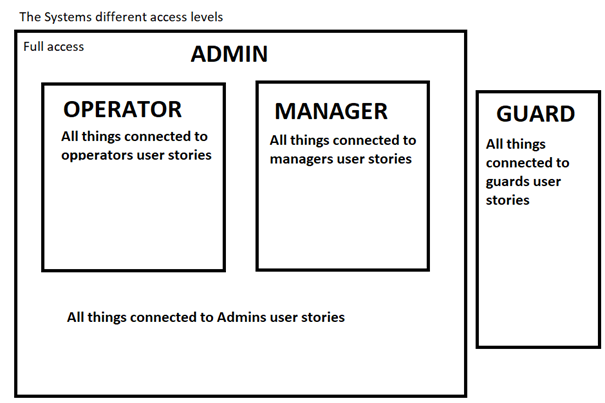
\includegraphics[width=0.6\textwidth]{TDDC88 - User Hierarchy.png}
    \caption{Visualization of user class hierarchy.}
    \label{fig:your_label}
\end{figure}

In practice the user classes and their functionality are as follows: 

\begin{itemize}

    \item \textbf{Guard:} the guard account only exists as a means to store data on the respective guard including username, name and email. The guard is then notified via the stored email address where they can view details of the alarm including a snapshot when an alarm is raised. The guards have no actual access to the web application.
    
    \item \textbf{Operator:} the operator account has access to the class specific alarm dashboard-page. Here the user can survey the system and most importantly receive notifications of when the system detects a potential intruder. After which they are able to either approve or dismiss alarms based on the snapshot provided by the camera and information such as camera ID, location e.t.c. They are also able to cancel active alarms through the dashboard.
    
    \item \textbf{Manager:} the account has access to the class specific statistics-page of the application where they can review the data of triggered alarms such as false- and true positives, dates and times e.t.c in order to take informed decisions on e.g. staff planning and camera locations. The lack access to the alarm dashboard-page of the operators.
    
    \item \textbf{Admin:} the account has access to both of the above operator and manager specific pages as well as an admin exclusive page where confidence level of the camera and scheduling of when the alarm system shall be active can be adjusted. Furthermore the admin has the ability to create accounts and adjust classes of existing accounts. As explained above, a master class of the application excluding the guard which is to be regarded as part of the system but not the application.
    
\end{itemize}


\subsubsection{Abbreviations}

\begin{itemize}
   \item \textbf{ACAP:} Axis Camera Application Platform, "An open application platform for software-based solutions built around Axis devices." \cite{ACAP}
     \item \textbf{GDPR:} General Data Protection Regulation,
"This regulation sets out provisions regarding the protection of natural persons in relation to the processing of personal data and the free movement of such data." \cite{GDPR}
\end{itemize}

\newpage

% Here you'll find information about the project
\section{Overall Description}

\subsection{Product Perspective}

\subsubsection{User Stories}

The following section outlines the desired functionality of the system based on various user classes and their interactions. These user stories describe the specific actions and expectations for Operators, Administrators, and Guards in managing the system effectively. Each story reflects the system's intended behavior in real-time surveillance and alarm management scenarios, ensuring a seamless and user-friendly experience.

Each user story is linked to functional and non-functional requirements based on their respective IDs.

 \begin{itemize}
 
    \item As an \textbf{Operator}, I want the system to recognize and classify objects and notify me when this is done to a 95\% confidence level, raising an alarm within 5 seconds by a clear user-friendly alert on the application dashboard. (Requirements: \hyperlink{FRQ001}{FRQ001-v1}, \hyperlink{FRQ003}{FRQ003-v1}, \hyperlink{FRQ013}{FRQ013-v1}, \hyperlink{NRQ005}{NRQ005-v1})
    
    \item When an alert of a detection is sent, the \textbf{Operator}, shall clearly be able to make an informed decision about if the alert should be dismissed or the alarm should be raised by displaying information about the location of the camera, the object identified, and a snapshot of the intruder. (Requirements: \hyperlink{FRQ002}{FRQ002-v1}, \hyperlink{FRQ005}{FRQ005-v1}, \hyperlink{NRQ002}{NRQ002-v1})
    
    \item As an \textbf{Operator}, if I approve that the alarm should be raised then the speaker should play the specified alarm sound and the email to the guard shall be sent within 5 seconds. If the alert is dismissed, then the time, date, and ID of the camera shall be stored in the database within 5 seconds. (Requirements: \hyperlink{FRQ004}{FRQ004-v1}, \hyperlink{FRQ015}{FRQ015-v1}, \hyperlink{NRQ002}{NRQ002-v1})
    
    \item As an \textbf{Operator}, I want to be able to access the live video feed from all cameras on demand, with a video feed visible within a maximum of 3 seconds after the button is pressed. This is to ensure correct camera placement and monitor situations in conjunction with raised alarms. (Requirements: \hyperlink{FRQ008}{FRQ008-v1}, \hyperlink{FRQ009}{FRQ009-v1})

    \item If an alarm is active, I, as an \textbf{Operator}, want to be able to cancel the alarm within 5 seconds at any time, resulting in the speaker turning off, the guard being notified of the cancellation, and the alarm data being stored in the database. (Requirements: \hyperlink{FRQ004}{FRQ004-v1}, \hyperlink{FRQ016}{FRQ016-v1}, \hyperlink{NRQ002}{NRQ002-v1})
    
    \item As a \textbf{Guard}, I want to receive a notification when an alarm is approved, specifying location, snapshot, and details about what to expect so I can be prepared to respond to security incidents. (Requirements: \hyperlink{FRQ002}{FRQ002-v1}, \hyperlink{FRQ015}{FRQ015-v1}, \hyperlink{NRQ002}{NRQ002-v1})

    \item As an \textbf{Admin}, I want to update the camera schedule and confidence level within 10 minutes of request, so I can manage operations efficiently and fine-tune object recognition. (Requirements: \hyperlink{FRQ006}{FRQ006-v1}, \hyperlink{FRQ007}{FRQ007-v1}, \hyperlink{NRQ003}{NRQ003-v1}, \hyperlink{NRQ004}{NRQ004-v1})

    \item As an \textbf{Admin}, I want the system to support multiple user categories (Operator, Manager, Admin), and I want to be able to configure the system so I can manage access levels for specific accounts and control system operations. (Requirements: \hyperlink{FRQ014}{FRQ014-v1}, \hyperlink{FRQ018}{FRQ018-v1}, \hyperlink{NRQ007}{NRQ007-v1})

    \item As a \textbf{Manager}, I want to see the number of alerts, the time of these alerts, location of these alerts, and if they were accurate and decided to require an alarm. I want to see this in a visual view, displaying these statistics as diagrams, for a clear overview. (Requirements: \hyperlink{FRQ010}{FRQ010-v1}, \hyperlink{FRQ011}{FRQ011-v1}, \hyperlink{FRQ012}{FRQ012-v1}, \hyperlink{FRQ017}{FRQ017-v1}, \hyperlink{NRQ005}{NRQ005-v1}, \hyperlink{NRQ006}{NRQ006-v1})
    
\end{itemize}

\subsection{Backlog}

This subsection ranks the user stories from highest priority to lowest priority. Difficulty means the effort required to fullfill a requirement on a scale from 1-5, with 5 being the most difficult. The ranking of difficulty is made by the developers and may change as the project proceeds.\\

\begin{table}[htbp]
\centering
\normalsize
\begin{tabular}{|c|p{10cm}|c|c|}
\hline
\textbf{User story ID} & \textbf{Description} & \textbf{Priority} & \textbf{Difficulty} \\
\hline
4 & As an Operator, I want the system to recognize and classify objects and notify me when this is done to a 95\% confidence level, raising an alarm within 5 seconds by a clear user-friendly alert on the application dashboard. & 1 & 4 \\
\hline
5 & When an alert of a detection is sent, the Operator shall clearly be able to make an informed decision about if the alert should be dismissed or the alarm should be raised by displaying information about the location of the camera, the object identified, and a snapshot of the intruder. & 2 & 2 \\
\hline
6 & As an Operator, if I approve that the alarm should be raised then the speaker should play the specified alarm sound and the email to the guard shall be sent within 5 seconds. If the alert is dismissed then the time, date, and ID of the camera shall be stored in the database within 5 seconds. & 3 & 3 \\
\hline
7 & As an Operator, I want to be able to access the live video feed from all cameras on demand, with a video feed visible within a maximum of 3 seconds after the button is pressed. This ensures correct camera placement and monitoring situations in conjunction with raised alarms. & 4 & 3 \\
\hline
1 & As a guard, I want to receive a notification when an alarm is approved, specifying location, snapshot, and details about what to expect so I can be prepared to respond to security incidents. & 5 & 1 \\
\hline
3 & As an admin, I want the system to support multiple user categories (Operator, Manager, Admin), and I want to be able to configure the system so I can manage access levels for specific accounts and control system operations. & 6 & 2 \\
\hline
8 & If an alarm is active, I, as an Operator, want to be able to cancel the alarm within 5 seconds at any time, resulting in the speaker turning off, the guard being notified of the cancellation, and the alarm data being stored in the database. & 7 & 3 \\
\hline
2 & As an admin, I want to update the camera schedule and confidence level within 10 minutes, so I can manage operations efficiently and fine-tune object recognition. & 8 & 3 \\
\hline
9 & As a manager, I want to see the number of alerts, the time of these alerts, the location of these alerts, and if they were accurate and decided to require an alarm. I want to see this in a visual view, displaying these statistics as diagrams for a clear overview. & 9 & 5 \\
\hline
\end{tabular}
\caption{User Stories with Priorities and Difficulty Levels}
\end{table}

\subsection{Product Functions}
The system will use the Axis camera and speaker to identify potential intruders. The software that will be developed will enable users to access different functionality such as alerts, camera settings and visual dashboards of the history. The concrete functions of the system will be: 

\begin{itemize}
    \item \textbf{Object Recognition:} The system shall recognize and classify objects in motion with a confidence level presented as a percentage. This feature uses advanced image processing algorithms built into the cameras to identify objects and determine their types.
    \item \textbf{Alerts to Operator:} Upon detecting a potential threat, the camera system will generate an alert that will be sent to the active operator. This alert includes sending images/videos, location and timestamp to the operational system and triggering an alarm if the threat is confirmed.
    \item \textbf{Alerts to Database:} Upon creating an alert, the timestamp, image/video, location and camera ID will be sent to the database.
    \item \textbf{Alarm Management:} Operators will have the ability to manage alarms by turning on or off the alarm system, including the speaker, and will have the option to confirm or deny the alarm based on the assessment of the displayed threat.
    \item \textbf{Scheduling Management:} Admin users will be able to configure and update the camera schedule. This function allows for flexible scheduling to ensure optimal camera coverage.
    \item \textbf{Confidence Adjustment:} Admin users will be able to adjust the camera’s confidence level. This allows for fine-tuning of the object recognition system to improve accuracy.
    \item \textbf{Live Camera Feeds:} Operators will have access to live feeds from active cameras, including their locations, to monitor real-time activities.
    \item \textbf{User Interface Navigation:} The system will provide an intuitive interface for operators to navigate through active camera feeds and manage alert responses effectively.
    \item \textbf{Alert Visualization:} Managers will have access to visual representations of alerts as data points, including the number of alerts, their locations, and timestamps. This data will be displayed in diagrams for easy analysis.
    \item \textbf{Alert Notifications Operator:} The system will visually indicate when an alert occurs through pop-ups or window changes, ensuring that operators are promptly informed.
    \item \textbf{User Management:} The system will support multiple user categories (Guard, Operator, Manager, Admin) with different access levels and capabilities. This includes the ability to manage user permissions and classes.
    \item \textbf{Integration and Accessibility:} The system will include standard pages such as login, user profile management, and system configuration to ensure ease of use and accessibility for authorized users.
\end{itemize}

\subsection{General Constraints}
Since Company 3 consists of 27 employees from with varying competences, it requires effective coordination and task allocation to leverage the specialized knowledge of each discipline. Furthermore, one can assume that a significant amount of the time budget must be used on educating employees on areas of lacking expertise. 

The aforementioned time budget, presenting the largest constraint of the project, is a strict limit of 160 hours per employee. This necessitates efficient time management, prioritization of tasks, and the implementation of streamlined processes to ensure that the project is completed within the available time frame. 

The nature of the company operating within the boundaries of a university course create other certain time constraints that the company must adhear to. This includes strict deadlines of iterations, pre-planned meetings, assignments e.tc. which limit the possibility of true to life operations and consumes a portion of the total time budget. 

\subsection{Assumptions and Dependencies}
The following assumptions have been made of the system, its users and customers:

\subsubsection{Installation of Cameras and Networking}
Company 3 delimits itself from responsibility in any part of either the installation of the cameras nor the networking that would be needed for application for an end-customer. The construction of the system will take little to no regard to ease of first installation, instead focusing on the usability of a pre-installed system.

\subsubsection{Staff Planning}
One of the systems key functionality will be to provide the manager statistics to create cost effective staff planning of the security system. This functionality will be based on historic data from the used camera, and will be displayed in a functional diagram to create a visual tool for the user to interpret.

\subsubsection{Dashboard Monitoring}
Company 3 assumes that the dashboard of the system will be monitored constantly by the end customers staff to take informed decisions on the alarms. This means that we will not send automatic notifications to guards in case of a lack of action on triggered alarms.

\subsection{Lower Ambition Levels}
To manage risks related to the time budget or other resource constraints, certain features or goals of this project may be considered for reduction or deferral. The before mentioned user stories represent the functionality that will be implemented, with a focus on usability, as per the customer's wishes. Beyond these user stories, some additional functional experiences may be added, depending on the available time, to further improve the delivered product. The following areas are identified as candidates for scope reduction without risking the delivered products functionality:

\subsubsection{Non-essential Features}
The user stories previously mentioned are describing the systems core functionality, in terms of viable time other good to have functionalities that could enhance the user experience or provide additional capabilities might be added. These are however not critical to the system's primary operations thereby not prioritised.

\subsubsection{Performance Optimization}
Enhancing the performance of a system should always be a goal of development, however minimum acceptable standards could be adjusted to meet budget constraints. As a base for the iteration the development team has set a standard success rate on 95 percent, but this will be further investigated through out the projects development. The code will however be designed to allow for addressing this in future iterations of the system. 

\subsubsection{Non-critical Testing}
Non-critical testing scenarios, such as edge cases or performance stress testing beyond expected operational loads, may be reduced to focus on core functional and usability testing. The main testing will be designed to confirm or deny the user stories previously mentioned. The main tests are further described in the testplan.

\newpage

% Here you'll find information about requirements
\section{Specific Requirements}

\subsection{Interface Requirements}
The system shall provide an interface which makes it easy to use and access. In order to achieve this the system shall have a cohesive graphic design when it comes to font, font size, header size, color scheme, page structure etc. The system shall have an interface which is intuitive to use such as standard pages in the application, i.e. login page, change information, start page and so on. Additionally, the user shall also be able to orient into active camera feeds and to dashboards presenting statistics. 


\subsection{Functional Requirements}
The system provides different functionality depending on the access level of the current user. User types follow a hierarchical structure, where each successive level grants increased access compared to the one before. The master class of admin, will have full access to the system. This will allow admins to set up new accounts, add cameras, adjust scheduling and adjust access. 

The camera will detect objects in motion, and based on the current confidence level and selected threat types, an alert will be sent to the operator. The camera will also record  timestamp, location, and capture a snapshot or video, which will be stored in a database. The operator will assess the alert and determine the appropriate course of action. If the alert is confirmed as a genuine threat, it will be marked as "verified" which triggers an alarm. For verified threats, the operator will notify a guard providing them with the timestamp, location, and key imagery from the incident. 

The system will include a page dedicated to displaying statistics, accessible by the supervisor. This page will retrieve data from the database and display the number of alerts, their locations, and timestamps in a diagram. 
\clearpage
\begin{table}[h]
\centering
\begin{tabular}{|l|p{8cm}|p{5cm}|}
\hline
\textbf{ID} & \textbf{Description} & \textbf{Sub-requirements} \\
\hline
\hypertarget{FRQ001}{FRQ001-v1} & The camera system shall recognize objects in motion and define what they are with a confidence presented as a percentage. & 
\hyperlink{01-1}{01-1}, \hyperlink{01-2}{01-2}, \hyperlink{01-3}{01-3} \\
\hline
\hypertarget{FRQ002}{FRQ002-v1} & The camera system shall send images to the external server if it is triggered. & 
\hyperlink{02-1}{02-1}, \hyperlink{02-2}{02-2}, \hyperlink{02-3}{02-3}, \hyperlink{02-4}{02-4} \\
\hline
\hypertarget{FRQ003}{FRQ003-v1} & The operational system shall alert the operator of an intrusion within 5 seconds of detection. & 
\hyperlink{03-1}{03-1}, \hyperlink{03-2}{03-2}, \hyperlink{03-3}{03-3}, \hyperlink{03-4}{03-4}, \hyperlink{03-5}{03-5} \\
\hline
\hypertarget{FRQ004}{FRQ004-v1} & The operational system shall enable the operator to turn off the alarm (including the speaker) at any time. & 
\hyperlink{04-1}{04-1}, \hyperlink{04-2}{04-2}, \hyperlink{04-3}{04-3}, \hyperlink{04-4}{04-4} \\
\hline
\hypertarget{FRQ005}{FRQ005-v1} & The operational system shall display the option to either confirm or deny an alarm. & 
\hyperlink{05-1}{05-1}, \hyperlink{05-2}{05-2}, \hyperlink{05-3}{05-3}, \hyperlink{05-4}{05-4} \\
\hline
\hypertarget{FRQ006}{FRQ006-v1} & The admin shall be able to update the camera schedule within 10 minutes 95\% of the time. & 
\hyperlink{06-1}{06-1}, \hyperlink{06-2}{06-2}, \hyperlink{06-3}{06-3}, \hyperlink{06-4}{06-4}, \hyperlink{06-5}{06-5} \\
\hline
\hypertarget{FRQ007}{FRQ007-v1} & The admin shall be able to update the camera confidence within 10 minutes 95\% of the time. & 
\hyperlink{07-1}{07-1}, \hyperlink{07-2}{07-2}, \hyperlink{07-3}{07-3} \\
\hline
\hypertarget{FRQ008}{FRQ008-v1} & The operator shall be able to see active cameras and their locations live. & 
\hyperlink{08-1}{08-1}, \hyperlink{08-2}{08-2}, \hyperlink{08-3}{08-3}, \hyperlink{08-4}{08-4} \\
\hline
\hypertarget{FRQ009}{FRQ009-v1} & The operator shall be able to orient into "active camera feeds." & 
\hyperlink{09-1}{08-2}, \hyperlink{09-2}{08-3}, \hyperlink{09-3}{08-4} \\
\hline
\hypertarget{FRQ010}{FRQ010-v1} & The manager shall be able to see the time of alerts in a diagram. & 
\hyperlink{10-1}{10-1}, \hyperlink{10-2}{10-2}, \hyperlink{10-3}{10-3}, \hyperlink{10-4}{10-4}, \hyperlink{10-5}{10-5} \\
\hline
\hypertarget{FRQ012}{FRQ012-v1} & The system shall have 4 different user categories, with different access levels (Guard, Operator, Manager, Admin). & 
\hyperlink{12-1}{12-1}, \hyperlink{12-2}{12-2}, \hyperlink{12-3}{12-3}, \hyperlink{12-4}{12-4} \\
\hline
\hypertarget{FRQ013}{FRQ013-v1} & The guard shall be alerted if the operator approves the alarm on a mobile unit. & 
\hyperlink{13-1}{13-1} \\
\hline
\hypertarget{FRQ014}{FRQ014-v1} & The manager shall be able to see statistics and alarm analysis. & 
\hyperlink{14-1}{14-1}, \hyperlink{14-2}{14-2} \\
\hline
\hypertarget{FRQ015}{FRQ015-v1} & The admin shall be able to manage the users. & 
\hyperlink{15-1}{15-1}, \hyperlink{15-2}{15-2} \\
\hline
\end{tabular}
\caption{Ordered Functional Requirements with clickable linked Sub-requirements}
\label{table:requirements_ordered}
\end{table}




 






\subsection{Non-functional Requirements}
The system shall have an encrypted and protected database storing data connected to triggered alarms including date, time, location and a comment.  

    The admin shall be able to schedule when the cameras will be active and inactive and this shall compile within a reasonable amount of time.  It shall also be possible for the admin to update the confidence level in the cameras without a noticeable delay in the system.   

The system as a whole shall be intuitivly to use, its design will be based on the principles availability, clarity, recognition, credibility and relevance, and to asses the intuitivness system usability scale (SUS) will be used as a tool. The system will be tested according to the test plan, where SUS is one of the msanual test for the product \cite{usabiltyPrinciples}. 

\begin{table}[h!]
\centering
\begin{tabular}{|l|p{8cm}|p{5cm}|}
\hline
\textbf{ID} & \textbf{Description} & \textbf{Implementation Plan} \\
\hline
\hypertarget{NRQ002}{NRQ002-v1} & The database shall store data about triggered alarms, including date, time, location, camera ID, and approved alarm or not (boolean). & 
\hyperlink{N02-1}{N02-1}, \hyperlink{N02-2}{N02-2}, \hyperlink{N02-3}{N02-3}, \hyperlink{N02-4}{N02-4}, \hyperlink{N02-5}{N02-5}, \hyperlink{N02-6}{N02-6} \\
\hline
\hypertarget{NRQ005}{NRQ005-v1} & The system shall have a cohesive graphic design (Font, Font size, header size, color scheme, page structure...). & 
\hyperlink{N05-1}{N05-1} \\
\hline
\hypertarget{NRQ007}{NRQ007-v1} & The system shall have different pages in the application. & 
\hyperlink{N07-1}{N07-1}, \hyperlink{N07-2}{N07-2}, \hyperlink{N07-3}{N07-3}, \hyperlink{N07-4}{N07-4} \\
\hline
\end{tabular}
\captionsetup{justification=centering}
\caption{Ordered Non-functional Requirements with clickable linked Sub-requirements}
\label{table:nonfunctional_requirements}
\end{table}

\clearpage

\subsection{Sub requirements}

The functional and non functional requirements have been broken down into more manageable tasks. These are connected to their respective requirement through the id, making tracing changes and understanding its motivation clear.

\begin{longtable}{|l|p{15cm}|}
\hline
\textbf{ID} & \textbf{Description} \\
\hline
\endfirsthead

\hline
\textbf{ID} & \textbf{Description} \\
\hline
\endhead

\hline \multicolumn{2}{|r|}{\textit{Continued on the next page}} \\
\hline
\endfoot

\hline
\endlastfoot

\hypertarget{02-1}{02-1} & The camera system shall output an image from the moment it is triggered. \\
\hline
\hypertarget{02-2}{02-2} & The camera system shall communicate with the external server. \\
\hline
\hypertarget{02-3}{02-3} & The camera system shall react if an alert is triggered. \\
\hline
\hypertarget{02-4}{02-4} & The camera system shall send the image, date, time, and location to the database. \\
\hline
\hypertarget{13-1}{13-1} & The guard shall be alerted in the form of an email. \\
\hline
\hypertarget{N02-1}{N02-1} & The database shall have all alarms sent to it. \\
\hline
\hypertarget{N02-2}{N02-2} & The database shall have a structure allowing time, date, location, and image. \\
\hline
\hypertarget{N02-3}{N02-3} & The database shall receive an alarm and save the information. \\
\hline
\hypertarget{N02-4}{N02-4} & The database shall be editable, allowing a change of status if the alarm was false. \\
\hline
\hypertarget{N02-5}{N02-5} & The database shall store an image only if the alarm was true for a maximum of 6 months. \\
\hline
\hypertarget{N02-6}{N02-6} & The database shall be connected with the WebUI, allowing retrieval of information. \\
\hline
\hypertarget{12-1}{12-1} & The guards shall not be able to access the application as they are only registered to store their contact info for notifications. \\
\hline
\hypertarget{12-2}{12-2} & The manager shall only be able to view statistics and not handle alarms. \\
\hline
\hypertarget{12-3}{12-3} & The operator shall only be able to handle alarms and not view statistics. \\
\hline
\hypertarget{12-4}{12-4} & The admin shall be able to use all the functionality of the application, including manager and operator functionality, system settings, and role handling. \\
\hline
\hypertarget{06-1}{06-1} & The admin shall have access to a WebUI showing the current schedule camera by camera. \\
\hline
\hypertarget{06-2}{06-2} & The admin shall have access to a WebUI allowing changes in the schedule. \\
\hline
\hypertarget{06-3}{06-3} & The camera schedule shall be updated within 10 minutes. \\
\hline
\hypertarget{06-4}{06-4} & The admin shall see these functions by entering each camera separately. \\
\hline
\hypertarget{06-5}{06-5} & The admin’s updates shall be performed 95\% of the time. \\
\hline
\hypertarget{07-1}{07-1} & The admin shall be able to view the camera’s chosen confidence. \\
\hline
\hypertarget{07-2}{07-2} & The admin shall see these functions by entering each camera separately. \\
\hline
\hypertarget{07-3}{07-3} & The admin shall be able to update the confidence within 10 minutes 95\% of the time. \\
\hline
\hypertarget{15-1}{15-1} & The admin shall be able to change the roles of users. \\
\hline
\hypertarget{15-2}{15-2} & The admin shall be able to remove the roles of users. \\
\hline
\hypertarget{N07-1}{N07-1} & The system shall have a statistics page (for managers and admins only). \\
\hline
\hypertarget{N07-2}{N07-2} & The system shall have a login page as a start page. \\
\hline
\hypertarget{N07-3}{N07-3} & The system shall have a start (landing) page. \\
\hline
\hypertarget{N07-4}{N07-4} & The system shall have a settings page (for admins only) where confidence levels of cameras can be changed and user roles managed. \\
\hline
\hypertarget{01-1}{01-1} & The camera shall output a variable showing what’s in front of it. \\
\hline
\hypertarget{01-2}{01-2} & The camera system shall give output of the confidence percentage for the recognized object. \\
\hline
\hypertarget{01-3}{01-3} & The camera shall send information to the external server. \\
\hline
\hypertarget{03-1}{03-1} & The operational system will receive information regarding alarms. \\
\hline
\hypertarget{03-2}{03-2} & The operational system will visually show the operator the alarm. \\
\hline
\hypertarget{03-3}{03-3} & The time from an alarm to it being visible for the operator shall be a maximum of 5 seconds. \\
\hline
\hypertarget{03-4}{03-4} & The operational system shall show the alarm as a pop-up. \\
\hline
\hypertarget{03-5}{03-5} & The pop-up shall disappear when handled. \\
\hline
\hypertarget{N05-1}{N05-1} & Wait for UX document. \\
\hline
\hypertarget{05-1}{05-1} & The operator will receive the alarm as a pop-up in the WebUI. \\
\hline
\hypertarget{05-2}{05-2} & The operator will decide on whether the alarm is true or false. \\
\hline
\hypertarget{05-3}{05-3} & The value of the operator’s decision will be added to the database statistics. \\
\hline
\hypertarget{05-4}{05-4} & The operator shall have the possibility to manually enter the cameras and decide to start an alarm (if wrongly triggered). \\
\hline
\hypertarget{04-1}{04-1} & The pop-up shall be a snapshot, location, time, and a choice to accept or dismiss the alarm. \\
\hline
\hypertarget{04-2}{04-2} & The operator shall have access to all active cameras and alarms. \\
\hline
\hypertarget{04-3}{04-3} & The operator shall have a button on the alarm that says "cancel alarm." \\
\hline
\hypertarget{04-4}{04-4} & The operator shall have a button on the alarm that says "start alarm." \\
\hline
\hypertarget{08-1}{08-1} & The operator shall be able to see all active cameras. \\
\hline
\hypertarget{08-2}{08-2} & Each camera shall have its confidence, schedule, and location visible. \\
\hline
\hypertarget{08-3}{08-3} & The operator shall be able to click on each active camera. \\
\hline
\hypertarget{08-4}{08-4} & The operator shall be able to click on an active camera feed. \\
\hline
\hypertarget{10-1}{10-1} & The manager shall have access to a site named "history." \\
\hline
\hypertarget{10-2}{10-2} & The site should display the relevant statistics. \\
\hline
\hypertarget{10-3}{10-3} & This should have get commands connected to the database. \\
\hline
\hypertarget{10-4}{10-4} & The manager shall be able to filter statistics. \\
\hline
\hypertarget{10-5}{10-5} & This site should have visual displays of the statistics. \\
\hline
\hypertarget{14-1}{14-1} & The system shall provide a page only accessible to managers and admins where statistics can be viewed. \\
\hline
\hypertarget{14-2}{14-2} & The system shall be able to receive alarm data (according to user story 9) and convert it into readable statistics. \\
\hline
\captionsetup{justification=centering}
\caption{Sub-Requirements with connected id}
\label{table:longtable}
\end{longtable}

\subsection{Design Constraints}


No significant design elements were requested by Axis Communications, which gives a degree of freedom to be more creative with the design approach. This flexibility allows room to explore various possibilities in terms of functionality and aesthetics, without being constrained by predefined requirements. However, while there is room to innovate, it is crucial that the system remains intuitive and user-friendly. The design shall be developed in iterations through close cooperation between developers, analysts and Axis Communications.

\newpage
¨% Here you'll find additional relevant info about the project



\printbibliography

\appendix
\section{Change Log}

\begin{longtable}{|l|p{8cm}|p{3cm}|}
\hline

\textbf{Section changed} & \textbf{Changes made} & \textbf{Who and when} \\
\hline
\endfirsthead

\hline
\textbf{Header 1} & \textbf{Header 2} & \textbf{Header 3} \\
\hline
\endhead

\hline \multicolumn{3}{|r|}{\textit{Continued on the next page}} \\
\hline
\endfoot

\hline
\endlastfoot
%Fill in changes here: 
Software System Attributes & Moved to architectural notebook. & William 15/10 \\
\hline
Limitation of User classes & Information moved to "user classes". & William 15/10 \\
\hline
Functional Requirements & Table added for new "subrequirements", link between these and functional requirements added in original table. & Melker 15/10. \\
\hline
\end{longtable} 

\end{document}

